\section*{Summary}

\subsection*{Process flow in scope}

The work will focus on out-of-hospital stroke patients who call for an ambulance, the system in scope is shown in figure \ref{fig:flow}.

\begin{figure}[h!]
\centering
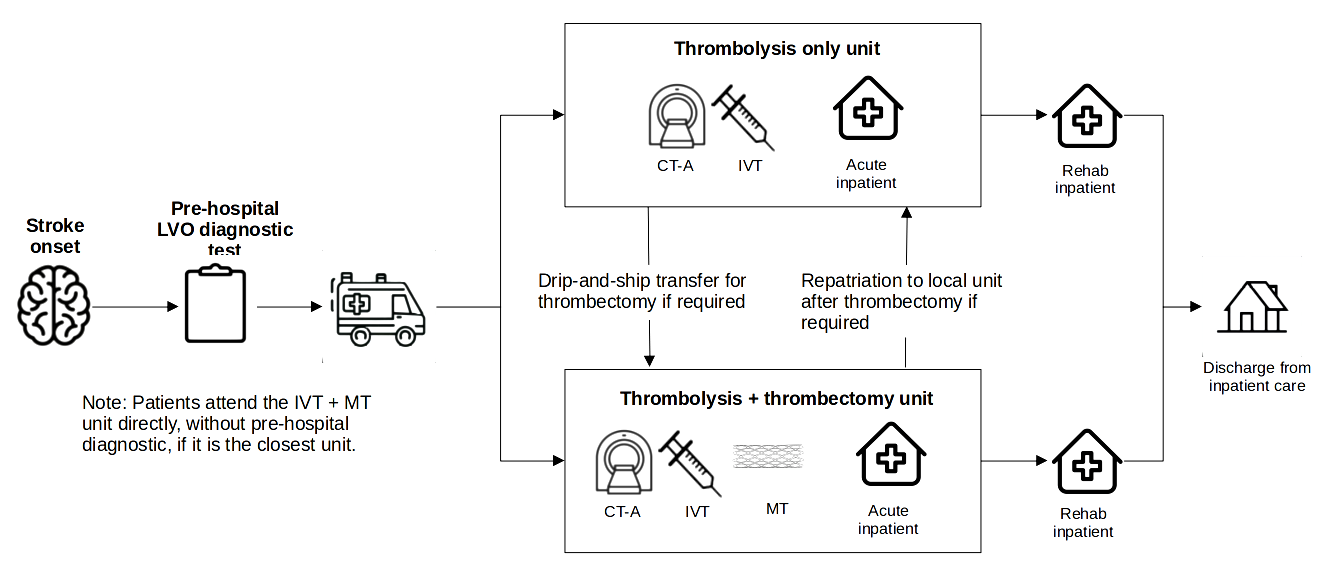
\includegraphics[width=1.0\textwidth]{./images/pathway}
\caption{Summary of patient flow through the emergency and in-patient rehabilitation stroke pathway.}
\label{fig:flow}
\end{figure}

\subsection*{Background}

The focus of our work is on using explainable machine learning and clinical pathway simulation, applied to national clinical audit data to identify between-hospital variation in clinical decision-making, and understanding the impact of that variation on patients and the health service. Our work is in collaboration with the Sentinel National Stroke Audit Programme and national and regional NHS bodies, which gives us a strong route into application of our modelling. We have focused mostly on the emergency stroke pathway, and variation in use of clot-busting drugs (the primary treatment of emergency stroke admissions).

In the proposed project we will bring multiple NIHR stroke-care project strands together in a single framework, and progress the modelling to include acute and rehabilitation in-patient care. We will investigate how variation in use of thrombolysis and thrombectomy will affect in-patient lengths of stay, and also investigate how in-patient lengths of stay vary between hospitals and regions, and how much of that variation is explained by differences in hospitals rather than differences in local stroke patient populations. As a result we will be able to evaluate how variation in clinical decision-making and processes effect both patient outcomes and bed requirements for in-patient stroke care. Additionally, we will include causal inference analysis that the team is developing. This will allow planners to see how an optimal system may behave in their area (e.g. at the level of integrated stroke delivery teams, or integrated care systems), and they may benchmark their performance against others, allowing for their own local patient population characteristics. Analysis and modelling will be made available through a web application.

The project will be a multi-methods study including machine learning, clinical pathway simulation, causal inference analysis, geographic modelling, and qualitative research. The team has the necessary skills and experience, with a well-established track-record, to undertake this work.

Figure \ref{fig:methods} shows a summary of the methods that will be integrated.

\begin{figure}[h!]
\centering
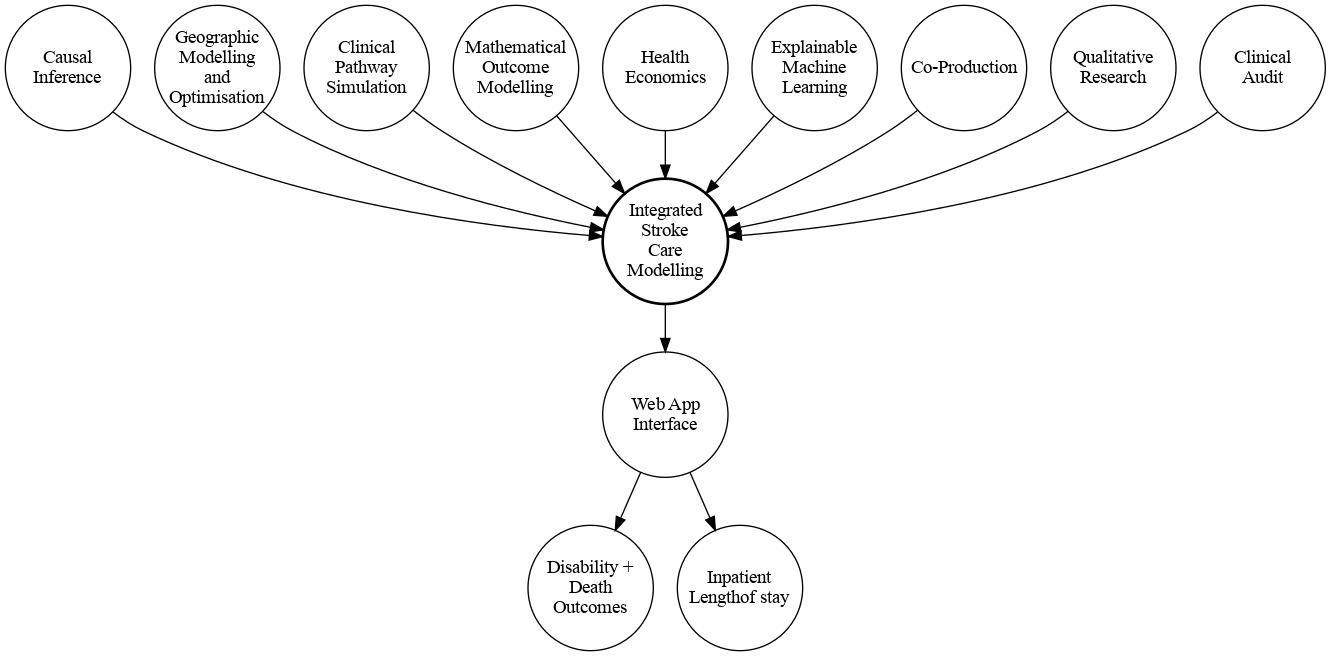
\includegraphics[width=1.0\textwidth]{./images/methods}
\caption{Summary of methods to be integrated for research and analysis output}
\label{fig:methods}
\end{figure}

\subsection*{Research questions}

\begin{enumerate}
    \item How much of the variation in inpatient length of stay comes from differences in local patient populations, and how much from differences in variation in clinical decision-making and processes?
    \item How would optimal provision of thrombolysis and thrombectomy (including pre-hospital processes, and decision-making on selecting suitable patients) affect outcomes and required stroke inpatient resources?
    \item Which predictors of best performance (outcomes and reduced lengths of stay) have good evidence that they are directly causal?
    \item Qualitative questions. \textbf{Need help here!} 
\end{enumerate}

